
%(BEGIN_QUESTION)
% Copyright 2011, Tony R. Kuphaldt, released under the Creative Commons Attribution License (v 1.0)
% This means you may do almost anything with this work of mine, so long as you give me proper credit

An antimicrobial agent called {\it acrolein} used to protect diesel fuel from fungal growth may be manufactured by reacting propylene with steam and air in a reactor vessel.  The ensuing chemical reaction is exothermic, and so a coolant loop using a special heat-transfer oil called ``Dowtherm'' is used to remove heat from the reactor vessel.  Suppose operators call you to troubleshoot a process problem they are having, and show you this graphic display on their control system monitor:

$$\includegraphics[width=15.5cm]{i03435x01.eps}$$

As you can see in this display, the temperature of the feed mixture into reactor R-23 is well below setpoint.  Based on the information found in this graphic display, help the operator identify the most likely cause of the underheated feed (from the list below), and explain why you chose the answer you did:

\vskip 10pt

\begin{itemize}
\item{} Control valve TV-101 mechanically stuck wide open
\item{} Water cooling tower turned off (not cooling water enough)
\item{} Control valve TV-99 mechanically stuck open
\item{} Heat exchanger E-77 poor heat transfer because of ``fouling'' on tubes
\item{} Control valve TV-99 mechanically stuck closed
\item{} Insufficient LP steam supply pressure/temperature 
\item{} Controller TC-99 left in manual mode
\item{} Dowtherm pump running too fast (flow too great)
\end{itemize}

\filbreak

\underbar{file i03435}
%(END_QUESTION)





%(BEGIN_ANSWER)

{\bf Insufficient LP steam supply pressure/temperature} is the most likely of the given causes, because it explains why the feed temperature into the reactor is well below setpoint while TV-101 is wide open.

\vskip 10pt

5 points for correct choice, 5 points for logical explanation.

%(END_ANSWER)





%(BEGIN_NOTES)

{\bf This question is intended for exams only and not worksheets!}.

%INDEX% Process: acrolein production 

%(END_NOTES)

